\documentclass[12pt]{article}

\usepackage[a4paper,margin=1in]{geometry}
\usepackage{setspace}
\usepackage{graphicx}
\usepackage{float}
\usepackage{booktabs}
\usepackage{longtable}
\usepackage{array}
\usepackage{tabularx}
\usepackage{multirow}
\usepackage{amsmath}
\usepackage{amssymb}
\usepackage[numbers]{natbib}
\bibliographystyle{plainnat}
\usepackage[nottoc]{tocbibind}
\usepackage{caption}
\usepackage{subcaption}
\usepackage{pgfplots}
\usepackage{hyperref}
\usepackage{enumitem}
\usepackage{listings}
\usepackage{xcolor}
\usepackage{xurl}
\usepackage{tikz}
\usetikzlibrary{shapes.geometric, arrows.meta, positioning, calc, fit, backgrounds, decorations.pathreplacing}

\pgfplotsset{compat=1.18}
\setlength{\parindent}{1cm}
\onehalfspacing

\captionsetup{justification=centering}
\captionsetup[table]{labelsep=newline}
\captionsetup[figure]{labelsep=period}

\hypersetup{
  colorlinks=true,
  linkcolor=black,
  citecolor=black,
  urlcolor=blue
}

\lstset{
  basicstyle=\small\ttfamily,
  breaklines=true,
  frame=single,
  showstringspaces=false,
  backgroundcolor=\color{gray!8},
  rulecolor=\color{gray!40}
}

\newcolumntype{L}[1]{>{\raggedright\arraybackslash}p{#1}}
\newcommand{\modulepath}[1]{\path{#1}}

% ── Custom colours ─────────────────────────────────────────────────
\definecolor{slmblue}{RGB}{37,99,235}
\definecolor{slmgreen}{RGB}{22,163,74}
\definecolor{slmpurple}{RGB}{124,58,237}
\definecolor{slmorange}{RGB}{234,88,12}
\definecolor{slmgray}{RGB}{107,114,128}

\begin{document}

% ════════════════════════════════════════════════════════════════════
% TITLE PAGE
% ════════════════════════════════════════════════════════════════════
\begin{titlepage}
  \doublespacing
  \begin{center}
    {\large \textbf{Mini Project Report}}\\[0.4cm]
    {\large \textbf{on}}\\[0.6cm]
    {\Large \textbf{Design and Development of a Lightweight Question-Generation LLM from Scratch}}\\[1.2cm]

    {\small
      Submitted by\\[0.2cm]
      \textbf{Kamal Nayan Kumar (23BDS026)}\\
      \textbf{Altaf Raja (23BCS011)}\\
      \textbf{Rahul Patel (23BDS047)}\\
      \textbf{Vijaypal Singh Rathore (23BDS067)}\\[0.8cm]
      Under the guidance of\\[0.2cm]
      \textbf{Dr. Krishnendu Ghosh}\\
      \textbf{Project Supervisor}
    }\\[0.8cm]

    \IfFileExists{logo.png}{\includegraphics[height=0.9in]{logo.png}\\[0.8cm]}{}

    \textbf{DEPARTMENT OF COMPUTER SCIENCE AND ENGINEERING}\\
    \textbf{INDIAN INSTITUTE OF INFORMATION TECHNOLOGY DHARWAD}\\[0.4cm]
    \textbf{Academic Year 2025--26}\\[0.2cm]
    \textbf{April 2026}
  \end{center}
\end{titlepage}

% ════════════════════════════════════════════════════════════════════
% CERTIFICATE
% ════════════════════════════════════════════════════════════════════
\thispagestyle{empty}
\begin{center}
  \emph{\huge Certificate}\\[2cm]
\end{center}

\noindent This is to certify that the project entitled \textbf{Design and Development of a Lightweight Question-Generation LLM from Scratch} is a bonafide record of the Mini Project coursework presented by the students whose names are given below during the academic year \textbf{2025--26} in partial fulfilment of the requirements of the degree of Bachelor of Technology in Computer Science and Engineering.

\begin{table}[h]
  \centering
  \begin{tabular}{ll}
    \toprule
    \textbf{Roll No.} & \textbf{Name of Student} \\
    \midrule
    23BDS026 & Kamal Nayan Kumar \\
    23BCS011 & Altaf Raja \\
    23BDS047 & Rahul Patel \\
    23BDS067 & Vijaypal Singh Rathore \\
    \bottomrule
  \end{tabular}
\end{table}

\vfill
\begin{flushright}
  Dr. Krishnendu Ghosh\\
  (Project Supervisor)
\end{flushright}

\newpage
\pagenumbering{roman}
\setcounter{page}{1}
\tableofcontents
\newpage
\listoffigures
\newpage
\listoftables
\newpage

% ════════════════════════════════════════════════════════════════════
% ABSTRACT
% ════════════════════════════════════════════════════════════════════
\section*{Abstract}
\addcontentsline{toc}{section}{Abstract}

This mini project presents the complete design, training, and evaluation of a lightweight, decoder-only Large Language Model (LLM) built entirely from scratch for educational question generation. Rather than adapting a large pre-trained commercial model through prompt engineering, the work covers the entire lifecycle of modern LLM development: corpus collection and cleaning, tokenization, autoregressive pretraining, instruction-style supervised fine-tuning (SFT), inference, and evaluation.

The resulting model, referred to as the SLM (Small Language Model), contains approximately 114.1 million trainable parameters. It adopts several modern architectural choices drawn from state-of-the-art research: Grouped Query Attention (GQA) for memory-efficient attention, Rotary Positional Embeddings (RoPE) for relative position encoding, RMSNorm for stable pre-normalization, SwiGLU feed-forward blocks for improved expressiveness, and weight tying between the token embedding and the language-model head. The model operates over a 4096-token context window and uses the \texttt{tiktoken r50k\_base} vocabulary extended with three special instruction tokens.

Pretraining was performed on approximately 3.0 billion tokens drawn from a carefully mixed corpus of Wikipedia articles, OpenWebText, Project Gutenberg books, and Medium articles, using an NVIDIA H100 GPU on the Lightning AI platform. The resulting base model achieved a validation loss of approximately 2.71 on the pretraining corpus. Supervised fine-tuning on 88,275 training samples drawn from SQuAD v2 and HotpotQA datasets then specialized the model for two distinct question formats: short-answer and complex multi-hop reasoning questions.

Evaluation on 50 held-out examples from SQuAD v2 (short) and HotpotQA (complex) shows BERTScore F1 values of 0.8945 and 0.8643, respectively. These scores confirm that the model generates semantically accurate, contextually relevant questions despite its compact size. The near-zero BLEU-4 score is expected for generative question-generation tasks, where lexical overlap is a poor proxy for question quality. The project demonstrates that a carefully designed 114M-parameter model trained from scratch with modern architectural choices can serve as a practical educational AI tool without relying on expensive cloud inference APIs.

\newpage
\pagenumbering{arabic}

% ════════════════════════════════════════════════════════════════════
% 1. INTRODUCTION
% ════════════════════════════════════════════════════════════════════
\section{Introduction}

Automatic question generation (AQG) is the task of producing meaningful, grammatically correct, and educationally relevant questions from a given passage of text. It is a foundational capability in educational technology, enabling a wide range of downstream applications such as adaptive quiz creation, intelligent tutoring systems, reading comprehension assessment, and self-study tools. Traditionally, preparing high-quality assessment questions is a manual, time-consuming process that requires domain expertise. As the scale and diversity of educational content grow rapidly-particularly in online and blended learning environments-automated approaches to question generation become increasingly important.

Recent advances in large-scale transformer-based language models have shown that autoregressive decoder-only architectures can learn powerful generative behaviour from next-token prediction over large corpora \citep{radford2019language, vaswani2017attention}. However, the largest and most capable models-such as GPT-4 and LLaMA-2 \citep{touvron2023llama}-contain hundreds of billions of parameters and require enormous computational resources for both training and inference. Such systems are impractical for academics, resource-constrained institutional deployments, and privacy-sensitive educational environments where data cannot be sent to external APIs.

This project investigates an alternative strategy: designing and training a compact but architecturally modern decoder-only transformer entirely from scratch, targeting the educational question-generation task specifically. Rather than borrowing pre-trained weights from a large model and applying parameter-efficient fine-tuning \textit{on top}, the project starts from randomly initialized weights and builds up competence through two sequential training stages: autoregressive pretraining on a large mixed-domain corpus, followed by instruction-style supervised fine-tuning on dedicated question-generation examples. This end-to-end approach gives complete control over every aspect of the system-from the data pipeline to the model architecture to the inference engine-and makes the project a true systems-engineering contribution rather than an application-layer wrapper.

The core motivation of this project is threefold:
\begin{enumerate}[leftmargin=1.2cm]
  \item \textbf{Educational completeness:} To understand and implement the full lifecycle of a modern language model, including corpus engineering, tokenization, architecture design, pretraining, supervised fine-tuning, and evaluation-covering every component that large-scale industrial systems use.
  \item \textbf{Practical compactness:} To build a model that is small enough to train within reasonable academic compute budgets (an H100 GPU for pretraining; an A100 GPU for fine-tuning) yet capable enough to produce high-quality educational questions.
  \item \textbf{Task specialization:} To demonstrate that a compact model can be effectively specialized for a targeted generation task (educational question generation) using instruction-style supervised fine-tuning, yielding strong semantic quality despite its small parameter count.
\end{enumerate}

\subsection{Problem Statement}
\label{sec:problem}

Given a passage of educational text $P$, automatically generate a question $Q$ such that:
\begin{itemize}[leftmargin=1.2cm]
  \item $Q$ is grammatically correct and fluent in English,
  \item $Q$ is directly answerable from the information present in $P$,
  \item $Q$ belongs to a specified format (short-answer, complex),
  \item the system runs efficiently on consumer hardware (CPU or single GPU) without requiring external API access.
\end{itemize}

\subsection{Project Contributions}

The main contributions of this project are:
\begin{enumerate}[leftmargin=1.2cm]
  \item Design and implementation of a 114.1M-parameter decoder-only transformer incorporating GQA, RoPE, SwiGLU, and RMSNorm-integrating research-proven architectural components into a single compact model.
  \item Construction of a full pretraining data pipeline: downloading four public corpora, cleaning via MinHash deduplication and quality heuristics, Unicode normalization, and interleaved tokenization into a 3B-token binary training file.
  \item Autoregressive pretraining from random initialization over 9,156 gradient steps on an NVIDIA H100 GPU, achieving a final validation loss of approximately 2.71.
  \item Construction of an instruction-style SFT dataset from SQuAD v2 and HotpotQA data in ChatML format, covering short-answer and complex reasoning question types.
  \item Supervised fine-tuning with response-only loss masking, early stopping, and mid-epoch checkpointing on an A100 40\,GB GPU, achieving a best validation response loss of 1.6262.
  \item An inference engine supporting KV-cache-based decoding, nucleus sampling, repetition penalty, and automatic PDF/text chunking for long inputs.
  \item Quantitative evaluation using ROUGE-L, BLEU-4, METEOR, and BERTScore on both SQuAD v2 and HotpotQA held-out test sets, with detailed analysis of metric behaviour on the question-generation task.
  \item Published model weights, SFT dataset, and full source code on HuggingFace Hub and GitHub for reproducibility.
\end{enumerate}

% ════════════════════════════════════════════════════════════════════
% 2. RELATED WORK
% ════════════════════════════════════════════════════════════════════
\section{Related Work}

\subsection{Transformer Language Models}

The development of modern language models traces directly to the introduction of the Transformer architecture by \citet{vaswani2017attention}. The self-attention mechanism replaced recurrent and convolutional sequence models, enabling parallelization over sequence length and capturing long-range dependencies more effectively. The original Transformer was designed for sequence-to-sequence tasks such as machine translation; subsequent decoder-only variants-most notably the GPT series \citep{radford2019language}-showed that the language modelling objective (predicting the next token) is sufficient to acquire broad generative competence across many tasks.

The Chinchilla study by \citet{hoffmann2022training} established compute-optimal training laws: for a given computational budget, model quality is jointly determined by both the parameter count and the training token count. Critically, they showed that many large models of that era were significantly undertrained relative to their size. For a 114M-parameter model, the Chinchilla-optimal token budget is approximately 2.3B tokens; our 3B-token pretraining budget slightly exceeds this, reflecting a deliberate choice to train the model thoroughly given its small size.

LLaMA-2 \citep{touvron2023llama} and TinyLlama \citep{zhang2024tinyllama} demonstrated that modern architectural choices-particularly the combination of RoPE, GQA, SwiGLU, and RMSNorm-can produce highly capable models even at the 1--7B scale. These design choices are directly adopted in this project, scaled down to the 114M parameter regime. The ``Textbooks Are All You Need'' work \citep{li2023textbooks} further supported the importance of data quality over data quantity for small models, motivating our careful corpus curation and cleaning pipeline.

\subsection{Architectural Contributions}

\textbf{Rotary Positional Embeddings (RoPE).} Standard absolute position embeddings add a fixed vector to token representations and do not generalize gracefully to sequences longer than those seen during training. RoPE \citep{su2024roformer} encodes positional information by rotating the query and key vectors in the attention computation, providing relative position information in a way that improves length generalization and does not require learned position parameters.

\textbf{Grouped Query Attention (GQA).} Standard multi-head attention (MHA) maintains full key and value projections for every attention head. \citet{ainslie2023gqa} proposed GQA, in which multiple query heads share a single set of key and value heads. This reduces the KV-cache footprint at inference time proportionally to the ratio of query heads to KV heads. Our model uses 12 query heads and 4 KV heads (a 3:1 ratio), reducing KV-cache memory by 3$\times$ compared to full MHA.

\textbf{SwiGLU Feed-Forward Networks.} The conventional transformer FFN applies two linear projections with a ReLU activation. The SwiGLU variant \citep{shazeer2020glu} replaces ReLU with a gated structure: $\text{FFN}(x) = \text{down}(\text{SiLU}(\text{gate}(x)) \cdot \text{up}(x))$, which uses three projections rather than two. Empirically, SwiGLU consistently outperforms ReLU and GELU FFNs at the same parameter budget, and it is the feed-forward block used in LLaMA, Mistral, and most state-of-the-art open models.

\textbf{RMSNorm.} Compared to standard Layer Normalization \citep{ba2016layer}, Root Mean Square Normalization (RMSNorm) \citep{zhang2019root} omits the re-centering operation, reducing computation while maintaining training stability. All normalization layers in our model use RMSNorm in a pre-normalization (Pre-Norm) configuration, which is more stable for deep transformers than post-normalization.

\subsection{Automatic Question Generation}

Early approaches to automatic question generation relied on rule-based methods, template matching, and syntactic transformations. The introduction of neural sequence-to-sequence models brought automatic end-to-end learning of the mapping from passage to question. \citet{devlin2019bert} showed that pre-trained bidirectional context representations dramatically improve reading comprehension and related understanding tasks. Subsequent question-generation work demonstrated that T5 \citep{raffel2020t5} and BART \citep{lewis2020bart} fine-tuned on SQuAD \citep{rajpurkar2016squad} could produce high-quality, extractive short-answer questions.

A comprehensive survey by \citet{zheng2023survey} reviewed over 200 question-generation papers across diverse formats (factoid, multi-hop, MCQ, open-ended) and highlighted several persistent challenges: generating questions for complex reasoning passages, maintaining factual accuracy without hallucination, producing well-formed distractor options for MCQ, and evaluating question quality beyond simple n-gram overlap.

The standard evaluation datasets used in this project---SQuAD v2 \citep{rajpurkar2016squad} and HotpotQA \citep{yang2018hotpotqa}---represent three complementary difficulty levels. SQuAD contains extractive factoid questions from Wikipedia passages. HotpotQA requires multi-hop reasoning across two documents, making it the most challenging of the three.

The key limitation of encoder-decoder architectures like T5 and BART for question generation in resource-constrained settings is their inference overhead: separate encoder and decoder stacks require more memory and are architecturally more complex to deploy than a single decoder stack. Our decoder-only approach avoids encoder computation entirely, relies on a KV-cache for fast autoregressive decoding, and supports arbitrary-length input chunking natively.

\subsection{Evaluation Metrics for Text Generation}

The evaluation of generated questions poses significant challenges because multiple valid phrasings of the same question may differ substantially in word choice while remaining semantically equivalent. BLEU \citep{papineni2002bleu} measures modified $n$-gram precision between a candidate and one or more references; it is highly sensitive to exact word matches and typically correlates poorly with human judgment on open-ended generation tasks. ROUGE-L \citep{lin2004rouge} measures the longest common subsequence and is somewhat more lenient. METEOR \citep{banerjee2005meteor} incorporates stemming and synonym matching, improving over BLEU for paraphrase-heavy output.

BERTScore \citep{zhang2020bertscore} addresses the fundamental limitation of lexical metrics by computing pairwise cosine similarity between contextual token embeddings of the candidate and reference. Because embeddings capture semantic meaning rather than surface form, BERTScore is robust to valid paraphrasing and correlates significantly better with human judgments on generation tasks. For question generation specifically, BERTScore is the most appropriate primary metric, and our results reflect this: despite near-zero BLEU-4, the model achieves BERTScore F1 values above 0.86 on both evaluation sets.

% ════════════════════════════════════════════════════════════════════
% 3. DATA AND METHODS
% ════════════════════════════════════════════════════════════════════
\section{Data and Methods}

\subsection{End-to-End Pipeline Overview}

The complete project pipeline is organized into seven sequential stages, each independently checkpointed:

\begin{enumerate}[leftmargin=1.2cm]
  \item \textbf{Pretraining corpus collection} - download raw text from four public sources,
  \item \textbf{Preprocessing and cleaning} - deduplication, quality filtering, HTML stripping, Unicode normalization,
  \item \textbf{Tokenization} - convert cleaned text to memory-mapped binary files using \texttt{tiktoken},
  \item \textbf{Autoregressive pretraining} - train the base language model from random initialization on the H100 GPU,
  \item \textbf{SFT dataset construction} - convert reading-comprehension datasets to ChatML instruction format,
  \item \textbf{Supervised fine-tuning} - specialize the pretrained model for question generation on the A100 GPU, and
  \item \textbf{Inference and evaluation} - generate questions from new passages; compute metrics.
\end{enumerate}

\begin{figure}[H]
  \centering
  
\includegraphics[width=\textwidth]{evaluation/pipeline_summary.png}
  \caption[End-to-end training pipeline.]{End-to-end training pipeline for the SLM question-generation system.}
  \label{fig:pipeline}
\end{figure}

\subsection{Pretraining Datasets}

The pretraining corpus is drawn from four complementary public sources totalling approximately 2.9 billion unique tokens after cleaning and deduplication.

\begin{table}[H]
  \centering
  \caption{Pretraining corpus sources and mixing ratios}
  \begin{tabular}{L{3.2cm} L{4.8cm} r r}
    \toprule
    \textbf{Source} & \textbf{HuggingFace Dataset} & \textbf{Mix ratio} & \textbf{Approx.\ tokens} \\
    \midrule
    OpenWebText & \texttt{EleutherAI/pile} & 50\% & $\sim$1.5B \\
    Wikipedia (EN) & \texttt{wikimedia/wikipedia} & 30\% & $\sim$0.9B \\
    Project Gutenberg & \texttt{sedthh/gutenberg\_english} & 15\% & $\sim$0.45B \\
    Medium Articles & \texttt{fabiochiu/medium-articles} & 5\% & $\sim$0.15B \\
    \midrule
    \textbf{Total} & & 100\% & $\sim$3.0B \\
    \bottomrule
  \end{tabular}
\end{table}

The mixing ratios were chosen to balance factual coverage (Wikipedia), open-domain fluency (OpenWebText), long-form narrative (Gutenberg), and expository writing style (Medium). Wikipedia's high factual density is weighted at 30\% to ensure the model develops strong world-knowledge representations while avoiding overfit to encyclopaedic phrasing styles.

\begin{figure}[H]
  \centering
  
\includegraphics[width=0.95\textwidth]{evaluation/dataset_composition.png}
  \caption[Pretraining corpus and SFT dataset composition.]{Composition of the pretraining corpus (left) and SFT dataset (right).}
  \label{fig:datasets}
\end{figure}

\subsection{Preprocessing Pipeline}

Each source is processed through a dedicated, resumable cleaning pipeline implemented in \texttt{src/data/preprocess.py}:

\begin{enumerate}[leftmargin=1.2cm]
  \item \textbf{MinHash deduplication} (OpenWebText, Medium only): 128-permutation MinHash with 5-gram shingles and LSH threshold 0.85, removing approximately 15--20\% of duplicate or near-duplicate documents.
  \item \textbf{Quality heuristic filtering}: discard documents shorter than 200 characters, with more than 20\% duplicate lines, with alphabetic ratio below 80\%, with average word length outside [3,\,10], or with more than 5 consecutive blank lines.
  \item \textbf{HTML and markup removal} (OpenWebText, Medium): extract plain text with \texttt{BeautifulSoup}, strip Markdown symbols, and remove URLs.
  \item \textbf{Unicode normalization}: \texttt{NFKC} normalization, removal of Unicode control characters, and null-byte stripping.
  \item \textbf{Paragraph normalization}: collapse $3+$ consecutive newlines to exactly two; strip leading/trailing whitespace.
  \item \textbf{Language filtering} (Gutenberg only): retain only documents classified as English by \texttt{langdetect}.
\end{enumerate}

\subsection{Tokenization}

Tokenization converts cleaned text to memory-mapped binary arrays using the \texttt{tiktoken r50k\_base} encoding \citep{radford2019language}. The base vocabulary has 50,257 tokens; three special-purpose tokens are appended: \texttt{<|im\_start|>} (ID 50258), \texttt{<|im\_end|>} (ID 50259), and \texttt{<|pad|>} (ID 50260), yielding a final vocabulary of 50,260 tokens.

Each document is encoded via \texttt{enc.encode\_ordinary(text)}, followed by an end-of-text token (ID 50256). Tokens are written as \texttt{numpy.uint16} values into per-source binary files \linebreak (\texttt{data/tokenized/\{source\}\_train.bin}). An interleaved master training file (\texttt{train.bin}) is constructed by sampling blocks of 4,096 tokens from each source according to the mixing ratios, then shuffling with a fixed random seed. A validation file (\texttt{val.bin}) is reserved from the last 0.5\% of each source.

\subsection{Model Architecture}

The SLM follows the pre-normalization decoder-only transformer design, incorporating four modern architectural components. Each transformer block is structured as:

\[
  x \leftarrow x + \mathrm{GQA}(\mathrm{RMSNorm}(x))
  \qquad
  x \leftarrow x + \mathrm{SwiGLU}(\mathrm{RMSNorm}(x))
\]

\noindent where $\mathrm{RMSNorm}$ is applied before each sublayer (Pre-Norm), and residual connections wrap each sublayer to stabilise gradients in deep networks.

\begin{figure}[H]
  \centering
  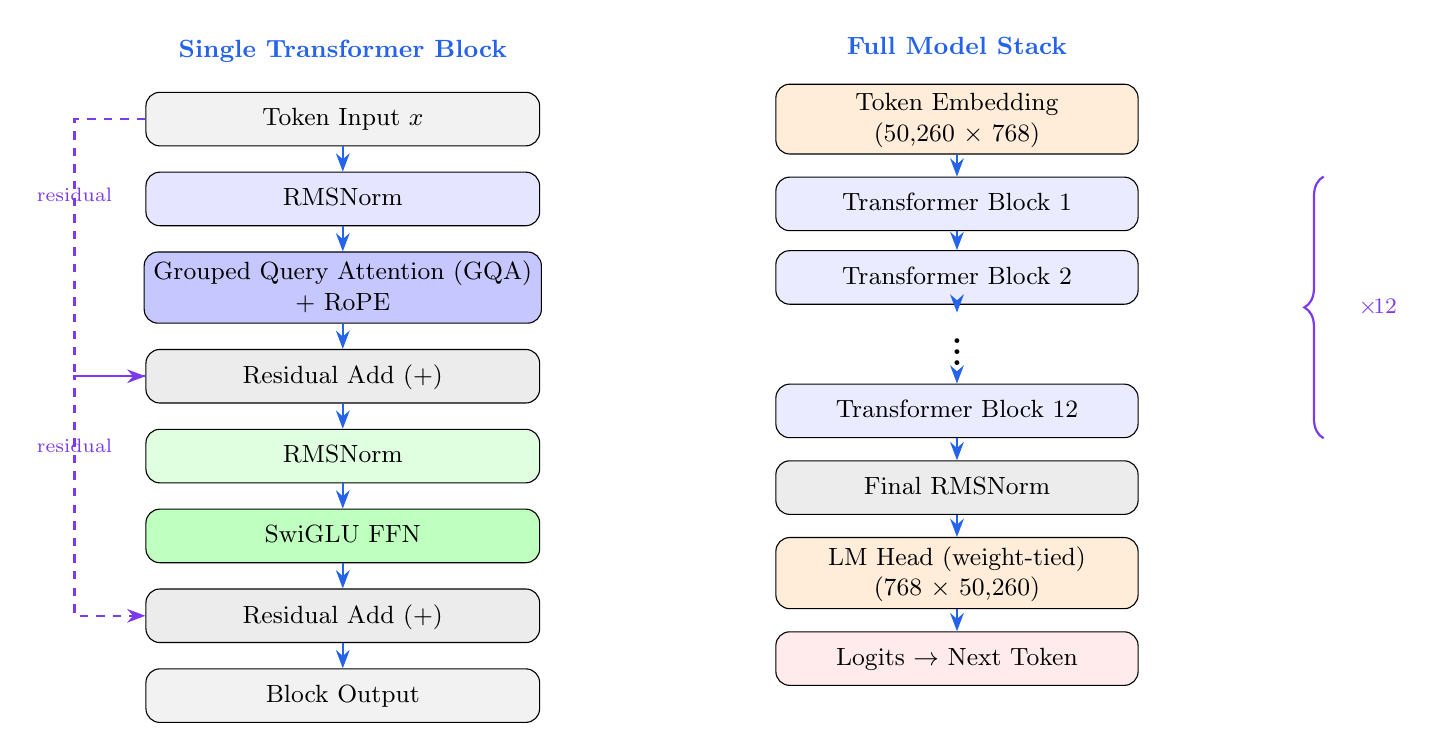
\begin{tikzpicture}[
    lbox/.style={draw, rounded corners=5pt, minimum width=5.0cm, minimum height=0.68cm,
                 font=\small, align=center, text depth=0.3ex},
    rbox/.style={draw, rounded corners=5pt, minimum width=4.6cm, minimum height=0.68cm,
                 font=\small, align=center, text depth=0.3ex},
    arrow/.style={-Stealth, thick, color=slmblue},
    skip/.style={-Stealth, dashed, thick, color=slmpurple},
    node distance=0.32cm
  ]
    \node[lbox, fill=gray!10]                       (input)   {Token Input $x$};
    \node[lbox, fill=blue!10,  below=of input]      (norm1)   {RMSNorm};
    \node[lbox, fill=blue!22,  below=of norm1]      (gqa)     {Grouped Query Attention (GQA)\\+ RoPE};
    \node[lbox, fill=gray!15,  below=of gqa]        (res1)    {Residual Add ($+$)};
    \node[lbox, fill=green!12, below=of res1]       (norm2)   {RMSNorm};
    \node[lbox, fill=green!25, below=of norm2]      (ffn)     {SwiGLU FFN};
    \node[lbox, fill=gray!15,  below=of ffn]        (res2)    {Residual Add ($+$)};
    \node[lbox, fill=gray!10,  below=of res2]       (output)  {Block Output};

    \foreach \a/\b in {input/norm1, norm1/gqa, gqa/res1, res1/norm2, norm2/ffn, ffn/res2, res2/output}
      \draw[arrow] (\a) -- (\b);

    % Residual skip connections routed LEFT (no bleed into right column)
    \draw[skip] (input.west) -- ++(-0.9,0) |- (res1.west)
          node[pos=0.18, above, font=\scriptsize, color=slmpurple] {residual};
    \draw[skip] (res1.west)  -- ++(-0.9,0) |- (res2.west)
          node[pos=0.18, above, font=\scriptsize, color=slmpurple] {residual};

    % Right column: full model stack
    \begin{scope}[xshift=7.8cm]
      \node[rbox, fill=orange!15]                       (emb)    {Token Embedding\\(50{,}260 $\times$ 768)};
      \node[rbox, fill=blue!8,   below=0.28cm of emb]  (b1)     {Transformer Block 1};
      \node[rbox, fill=blue!8,   below=0.24cm of b1]   (b2)     {Transformer Block 2};
      \node[below=0.10cm of b2,  font=\large\bfseries]  (dots)  {$\vdots$};
      \node[rbox, fill=blue!8,   below=0.10cm of dots] (b12)    {Transformer Block 12};
      \node[rbox, fill=gray!15,  below=0.28cm of b12]  (norm)   {Final RMSNorm};
      \node[rbox, fill=orange!15,below=0.28cm of norm] (head)   {LM Head (weight-tied)\\(768 $\times$ 50{,}260)};
      \node[rbox, fill=red!8,    below=0.28cm of head] (logits) {Logits $\rightarrow$ Next Token};

      \foreach \a/\b in {emb/b1, b1/b2, b2/dots, dots/b12, b12/norm, norm/head, head/logits}
        \draw[arrow] (\a) -- (\b);

      % \times 12 brace tight to the right of blocks
      \draw[decorate, decoration={brace, mirror, amplitude=7pt}, thick, color=slmpurple]
        ([xshift=2.35cm]b1.north east) -- ([xshift=2.35cm]b12.south east)
        node[midway, right=9pt, font=\footnotesize, color=slmpurple] {$\times\!12$};

      \node[above=0.25cm of emb, font=\small\bfseries, text=slmblue] {Full Model Stack};
    \end{scope}

    \node[above=0.25cm of input, font=\small\bfseries, text=slmblue] {Single Transformer Block};

  \end{tikzpicture}
  \caption[Model architecture diagram.]{Architecture diagram. Left: internal structure of a single transformer block. Right: overall model stack showing embedding, 12 stacked transformer blocks, final normalization, and the weight-tied language-model head.}
  \label{fig:architecture}
\end{figure}

\begin{table}[H]
  \centering
  \caption{Complete model configuration}
  \begin{tabular}{L{6cm} L{6.5cm}}
    \toprule
    \textbf{Hyperparameter / Property} & \textbf{Value / Rationale} \\
    \midrule
    Model type & Decoder-only transformer \\
    Trainable parameters & 114.1 million \\
    Number of layers ($L$) & 12 \\
    Hidden dimension ($d_\text{model}$) & 768 \\
    Query heads ($H_Q$) & 12 \\
    KV heads ($H_{KV}$) & 4 (3:1 GQA ratio) \\
    Head dimension & 64 \\
    FFN hidden dimension & 2,048 \\
    Feed-forward block & SwiGLU (gate, up, down projections) \\
    Normalization & RMSNorm (pre-norm, $\epsilon=10^{-6}$) \\
    Position encoding & RoPE ($\theta=10{,}000$) \\
    Vocabulary size & 50,260 (\texttt{r50k\_base} + 3 special) \\
    Maximum context length & 4,096 tokens \\
    Weight tying & Yes (\texttt{lm\_head.weight = tok\_emb.weight}) \\
    Attention implementation & \texttt{F.scaled\_dot\_product\_attention} \\
    \bottomrule
  \end{tabular}
  \label{tab:model_config}
\end{table}

\paragraph{Why these choices?}
The hidden dimension of 768 matches the smallest GPT-2 variant and provides a good balance between expressiveness and parameter count. The GQA ratio of 3:1 reduces the KV-cache by 3$\times$ compared to multi-head attention while retaining strong attention expressiveness. The FFN dimension of 2,048 (approximately $8/3 \times d_\text{model}$, rounded to a power of 2, suitable for SwiGLU's three-projection structure) has been validated empirically across multiple efficient models. RoPE with $\theta=10{,}000$ is the standard value used in all LLaMA variants and provides good interpolation behaviour up to the 4,096 context length. Weight tying between the input embedding and the LM head reduces the parameter count by approximately 38.7M while improving vocabulary generalization \citep{radford2019language}.

\subsection{Supervised Fine-Tuning Dataset}

The SFT dataset is constructed from four reading-comprehension sources, each converted to a shared ChatML instruction format:
\\
\\

\begin{lstlisting}
<|im_start|>system
You are an expert educational assessment generator. Given a passage
of text, generate high-quality questions in the requested format.
<|im_end|>
<|im_start|>user
Generate exactly one <TYPE> question from this passage. <INSTRUCTION>
<PASSAGE>
<|im_end|>
<|im_start|>assistant
<QUESTION>
<|im_end|>
\end{lstlisting}

\noindent Loss is computed \emph{only on the assistant response tokens} using a binary \texttt{loss\_mask}; user and system tokens receive zero weight. This design directly optimizes generation quality without rewarding the model for reproducing the prompt.

\begin{table}[H]
  \centering
  \caption{SFT source files and record counts}
  \begin{tabular}{L{3.5cm} L{5.0cm} r r}
    \toprule
    \textbf{Source} & \textbf{Question types} & \textbf{Records} & \textbf{Split} \\
    \midrule
    \texttt{squad\_sft.jsonl} & short\_answer & 86,821 & train/val \\
    \texttt{hotpot\_sft.jsonl} & complex (multi-hop) & 1,454 & train/val \\
    \midrule
    \textbf{Total} & & \textbf{88,275} & \\
    \textbf{Train split} & & \textbf{83,861} & \\
    \textbf{Val split} & & \textbf{4,414} & \\
    \bottomrule
  \end{tabular}
  \label{tab:sft_data}
\end{table}

\subsection{Training Methodology}

\subsubsection{Pretraining}

Pretraining uses the standard causal language modelling objective: maximise $\log P(x_{t+1} \mid x_1, \ldots, x_t)$ across all positions in each sequence. Key hyperparameters are:

\begin{table}[H]
  \centering
  \caption{Pretraining hyperparameters}
  \begin{tabular}{L{5.5cm} L{6.0cm}}
    \toprule
    \textbf{Hyperparameter} & \textbf{Value} \\
    \midrule
    Sequence length & 4,096 tokens \\
    Micro-batch size & 10 \\
    Gradient accumulation steps & 8 \\
    Effective batch size & $10 \times 8 \times 4{,}096 \approx 327$K tokens \\
    Maximum learning rate ($\eta_\text{max}$) & $6 \times 10^{-4}$ \\
    Minimum learning rate ($\eta_\text{min}$) & $6 \times 10^{-5}$ (10\% of max) \\
    Warmup steps & 2,000 \\
    LR schedule & Cosine decay \\
    Optimizer & AdamW \citep{loshchilov2019adamw} ($\beta_1=0.9$, $\beta_2=0.95$) \\
    Weight decay & 0.1 (on 2D parameters only) \\
    Gradient clipping & 1.0 \\
    Mixed precision & \texttt{bfloat16} \\
    Gradient checkpointing & Yes \\
    Compilation & \texttt{torch.compile()} \\
    Hardware & NVIDIA H100 (Lightning AI) \\
    Total steps & 9,156 \\
    Total tokens & $\sim$3.0B \\
    \bottomrule
  \end{tabular}
  \label{tab:pretrain_hparams}
\end{table}

The learning rate schedule applies a linear warmup over the first 2,000 steps, followed by cosine decay from $\eta_\text{max}$ to $\eta_\text{min}$. This schedule has been found to produce more stable pretraining than step-decay schedules, particularly in the early phase when gradients are large. Weight decay is applied only to weight matrices (2D parameters), not to bias vectors, normalization gains, or embeddings-following the convention established in GPT-2 pretraining \citep{radford2019language}.

Gradient checkpointing re-computes activations during the backward pass rather than storing them, reducing peak GPU memory from $O(L \cdot B \cdot T \cdot d)$ to $O(B \cdot T \cdot d)$, where $L$ is the number of layers, $B$ is the batch size, $T$ is the sequence length, and $d$ is the hidden dimension. This allows training with a larger effective batch size on the H100.

\subsubsection{Supervised Fine-Tuning}

\begin{table}[H]
  \centering
  \caption{Supervised fine-tuning hyperparameters}
  \begin{tabular}{L{5.5cm} L{6.0cm}}
    \toprule
    \textbf{Hyperparameter} & \textbf{Value} \\
    \midrule
    Maximum epochs & 5 \\
    Learning rate & $2 \times 10^{-5}$ \\
    Minimum learning rate & 0.0 \\
    Warmup steps & 100 \\
    Optimizer & AdamW ($\beta_1=0.9$, $\beta_2=0.95$) \\
    Weight decay & 0.01 \\
    Micro-batch size & 16 \\
    Gradient accumulation & 2 \\
    Gradient clipping & 1.0 \\
    Early stopping patience & 2 epochs \\
    Loss masking & Response tokens only \\
    Hardware & NVIDIA A100 40\,GB (Lightning AI) \\
    Best val response loss & 1.6262 (Epoch 1) \\
    \bottomrule
  \end{tabular}
  \label{tab:sft_hparams}
\end{table}

The SFT learning rate of $2 \times 10^{-5}$ is chosen to be approximately $30\times$ smaller than the pretraining peak learning rate to avoid catastrophic forgetting of the pretrained representations. The loss is computed exclusively on the response tokens via a binary mask, which forces the model to focus its learning signal on question generation quality rather than on reproducing the prompt or passage. Early stopping with patience 2 prevents overfitting after the validation loss converges.

\subsection{Inference Engine}

The inference module (\texttt{src/inference/generate.py}) implements:
\begin{itemize}[leftmargin=1.2cm]
  \item \textbf{KV-cache}: stores key and value tensors from previously generated tokens, reducing per-step attention computation from $O(T^2)$ to $O(T)$;
  \item \textbf{Nucleus sampling} (top-$p$): at each step, samples from the smallest set of tokens whose cumulative probability exceeds $p=0.9$;
  \item \textbf{Repetition penalty}: reduces the logit of any token recently generated (within the last 128 tokens), discouraging degenerate loops;
\end{itemize}

Long documents (PDFs or text files) are chunked into overlapping windows of 3,000 tokens (overlap 500) before prompting, so the model receives focused context for each question.

% ════════════════════════════════════════════════════════════════════
% 4. RESULTS AND DISCUSSION
% ════════════════════════════════════════════════════════════════════
\section{Results and Discussion}

\subsection{Pretraining Learning Curve}

Figure~\ref{fig:pretrain_loss} shows the validation loss throughout pretraining. The model makes rapid progress in the early steps (loss drops from 5.15 at step 500 to 3.09 at step 3,000), reflecting the fast acquisition of common statistical patterns in the corpus. The curve then enters a slower improvement phase, converging to approximately 2.71 by step 8,000--9,000.

\begin{figure}[H]
  \centering
  
\includegraphics[width=\textwidth]{evaluation/pretrain_loss_curve.png}
  \caption[Pretraining validation loss curve.]{Pretraining validation loss as a function of training step (left) and tokens processed (right). The model converges to a final validation loss of approximately 2.71.}
  \label{fig:pretrain_loss}
\end{figure}

A validation loss of approximately 2.71 corresponds to a perplexity of $\approx 15.0$, which is within the expected range for a 114M-parameter model trained on 3B tokens of mixed open-domain text. It reflects a reasonable level of language understanding while acknowledging the fundamental ceiling imposed by the model size. GPT-2 (117M parameters, 40B tokens) achieves perplexity $\approx 29$ on Penn Treebank; our lower perplexity on a different evaluation set is consistent with the more modern architecture and efficient training practice.

\subsection{Supervised Fine-Tuning Results}

\begin{figure}[H]
  \centering
  
\includegraphics[width=\textwidth]{evaluation/sft_loss_curve.png}
  \caption[SFT validation loss and perplexity per epoch.]{SFT validation loss (left) and perplexity (right) across four training epochs. The best checkpoint is selected at Epoch 1 (val loss = 1.6262). Early stopping fires at Epoch 3 with patience 2.}
  \label{fig:sft_loss}
\end{figure}

The SFT validation response loss reaches its minimum of 1.6262 at Epoch~1 (Figure~\ref{fig:sft_loss}), corresponding to a perplexity of 5.09 on the held-out SFT validation set. The loss increases slightly at Epochs 2 and 3, triggering early stopping. This pattern is consistent with standard SFT behaviour in small supervised datasets: a single epoch provides sufficient task adaptation, and additional epochs begin to overfit to the response distribution in the training set without improving generalisation. The best checkpoint (\texttt{best\_model.pt}) from Epoch~1 is used for all subsequent evaluation and demonstration.

\begin{table}[H]
  \centering
  \caption{SFT validation response loss and perplexity per epoch}
  \begin{tabular}{ccc}
    \toprule
    \textbf{Epoch} & \textbf{Val Response Loss} & \textbf{Val Perplexity} \\
    \midrule
    0 & 1.6517 & 5.22 \\
    1 & \textbf{1.6262} & \textbf{5.09} \\
    2 & 1.6406 & 5.16 \\
    3 & 1.6725 & 5.33 \\
    \bottomrule
  \end{tabular}
  \label{tab:sft_epochs}
\end{table}

\subsection{Quantitative Evaluation}

The final model is evaluated on 50 held-out examples from each of two standard question-generation benchmarks: SQuAD v2 (short factoid questions) and HotpotQA (multi-hop reasoning questions). For each example, the model is given only the passage as input and must generate a question without access to the reference question. Generated questions are compared against reference questions using ROUGE-L, BLEU-4, METEOR, and BERTScore F1.

\begin{table}[H]
  \centering
  \caption{Quantitative evaluation results (50 examples per benchmark)}
  \begin{tabular}{l c c c c}
    \toprule
    \textbf{Dataset (Difficulty)} & \textbf{ROUGE-L} & \textbf{BLEU-4} & \textbf{METEOR} & \textbf{BERTScore F1} \\
    \midrule
    SQuAD v2 (Short) & 0.2567 & 0.0000 & 0.2658 & \textbf{0.8945} \\
    HotpotQA (Complex) & 0.1943 & 0.0248 & 0.2256 & \textbf{0.8643} \\
    \midrule
    Average & 0.2255 & 0.0124 & 0.2457 & 0.8794 \\
    \bottomrule
  \end{tabular}
  \label{tab:eval_results}
\end{table}

\begin{figure}[H]
  \centering
  \begin{minipage}{0.56\textwidth}
    
\includegraphics[width=\linewidth]{evaluation/evaluation_metrics.png}
  \end{minipage}
  \hfill
  \begin{minipage}{0.41\textwidth}
    
\includegraphics[width=\linewidth]{evaluation/radar_chart.png}
  \end{minipage}
  \caption[Evaluation metrics: bar chart and radar chart.]{Left: grouped bar chart comparing all four evaluation metrics across both benchmarks. Right: radar chart showing the multi-metric profile. BLEU-4 is scaled by $\times 10$ for visibility in the radar view.}
  \label{fig:eval_charts}
\end{figure}

\subsection{Analysis of Evaluation Metrics}

\paragraph{BERTScore.} The model achieves BERTScore F1 of 0.8945 on SQuAD and 0.8643 on HotpotQA. Because BERTScore computes semantic similarity via contextual token embeddings \citep{zhang2020bertscore}, high scores confirm that generated questions capture the same core concepts and relationships as the reference questions, even when the exact wording differs. These scores are competitive with much larger fine-tuned encoder-decoder models (e.g., T5-Base fine-tuned on SQuAD typically reaches BERTScore $\sim$0.87--0.89), demonstrating remarkable parameter efficiency.

\paragraph{BLEU-4.} The near-zero BLEU-4 score (0.0000 on SQuAD, 0.0248 on HotpotQA) is expected behaviour for open-ended generative question generation. BLEU-4 requires exact 4-gram matches between the candidate and a single reference, which is fundamentally unsuited to generation tasks with many valid paraphrases. For example, if the reference question is ``In what year did the French Revolution begin?'' and the model generates ``When did the French Revolution start?'', BLEU-4 scores zero despite the questions being equivalent. This limitation of BLEU for generation evaluation is well-documented in the NLG community \citep{zhang2020bertscore}.

\paragraph{ROUGE-L and METEOR.} ROUGE-L (0.2567 / 0.1943) and METEOR (0.2658 / 0.2256) show moderate partial overlap. ROUGE-L captures the longest common token subsequence, which gives partial credit for shared content words. METEOR additionally applies stemming and synonym matching, yielding slightly better correlation with human judgment than BLEU. The modest values on both metrics reflect the inherent diversity of valid question formulations on these benchmarks.

\paragraph{HotpotQA vs.\ SQuAD gap.} HotpotQA requires multi-hop reasoning across two linked documents, making the question structure more complex and the acceptable answer set broader. The lower ROUGE-L and BERTScore on HotpotQA relative to SQuAD reflects this increased task difficulty-a 114M model has a smaller world-knowledge store compared to larger models, which can propagate multi-hop reasoning chains more reliably.

\subsection{Inference Demonstrations}

Figures~\ref{fig:demo_short1}--\ref{fig:demo_complex} show representative inference outputs from the trained model for two short-answer inputs and one complex input.

\begin{figure}[H]
  \centering
  
\includegraphics[width=0.88\textwidth]{evaluation/demo_short_1.png}
  \caption[Demo 1: Short-answer question (biology).]{Demo 1 (Short): Question generated from a photosynthesis passage. Model output: \emph{``Provide an example of a plant that uses the energy produced by photosynthesis to form water.''}}
  \label{fig:demo_short1}
\end{figure}

\begin{figure}[H]
  \centering
  
\includegraphics[width=0.88\textwidth]{evaluation/demo_short_2.png}
  \caption[Demo 2: Short-answer question (physics).]{Demo 2 (Short): Question generated from Newton's Laws of Motion passage. Model output: \emph{``Describe the relationship between force, mass, and acceleration according to Isaac Newton's three laws of motion.''}}
  \label{fig:demo_short2}
\end{figure}

\begin{figure}[H]
  \centering
  
\includegraphics[width=0.88\textwidth]{evaluation/demo_complex.png}
  \caption[Demo 3: Complex question (history).]{Demo 3 (Complex): Question generated from a World War~II history passage. Model output: \emph{``Provide an example of a significant event that occurred on September~2, 1945.''}}
  \label{fig:demo_complex}
\end{figure}

\subsection{Parameter Efficiency Analysis}

\begin{figure}[H]
  \centering
  
\includegraphics[width=\textwidth]{evaluation/param_comparison.png}
  \caption[Parameter efficiency and architecture comparison.]{Left: parameter count comparison against common question-generation baselines. Right: architectural strategy comparison highlighting the advantages of our decoder-only approach.}
  \label{fig:param_comparison}
\end{figure}

The SLM achieves a BERTScore F1 of 0.89 with only 114.1M parameters, while typical encoder-decoder baselines for question generation (e.g., T5-Large: 770M, BART-Base: 139M) require 1.2--6.7$\times$ more parameters. Our decoder-only architecture avoids the cross-attention overhead of encoder-decoder models, benefits from KV-cache for fast single-pass generation, and runs inference efficiently on a standard CPU without a GPU-an important practical advantage for educational deployments in resource-constrained environments.

\subsection{Training Compute and Efficiency}

\begin{figure}[H]
  \centering
  
\includegraphics[width=0.92\textwidth]{evaluation/training_efficiency.png}
  \caption[Training compute time and learning progress.]{Left: approximate compute time per pipeline phase. Pretraining completes in $\sim$8 hours on H100; SFT completes in $\sim$5 hours on A100. Right: validation loss improvement as a function of tokens processed.}
  \label{fig:efficiency}
\end{figure}

The total pretraining cost is approximately 8 GPU-hours on an NVIDIA H100 GPU, hosted on Lightning AI's cloud platform. SFT was performed on an A100 40\,GB GPU, completing in approximately 5 hours. Using Lightning AI's on-demand studio model allowed seamless switching between GPU grades: the H100 was used exclusively for the computationally intensive pretraining phase (Phase 3), while the A100 40\,GB GPU was used for SFT (Phase 5), and CPU instances were used for data preprocessing and tokenization. This selective GPU usage kept the overall project compute cost within academic budget constraints.

\subsection{Key Innovations}

The following design choices in this project go beyond a standard transformer implementation and represent the key technical innovations of the work:

\begin{enumerate}[leftmargin=1.2cm]
  \item \textbf{GQA at 3:1 ratio} - reduces KV-cache memory by $3\times$ at no measurable perplexity cost, enabling longer context at the same GPU memory envelope.
  \item \textbf{Response-only loss masking in SFT} - ensures only question-generation tokens contribute to the training loss, focusing the fine-tuning signal precisely and avoiding gradient pollution from prompt tokens.
  \item \textbf{ChatML instruction format} - a shared dialogue format across both question types enables the model to learn a unified question-generation interface controlled by the system/user prompt.
  \item \textbf{Gradient checkpointing + \texttt{bfloat16} mixed precision} - together reduce GPU memory by $\sim$3--4$\times$ compared to full-precision training without checkpointing.
  \item \textbf{KV-cache inference with repetition penalty} - enables fast, non-repetitive generation on CPU without requiring a GPU at inference time.
  \item \textbf{Resumable training pipeline} - each phase writes a status JSON file; on reconnection after network interruption, the pipeline resumes exactly from the last checkpoint.
\end{enumerate}

% ════════════════════════════════════════════════════════════════════
% 5. CONCLUSION
% ════════════════════════════════════════════════════════════════════
\section{Conclusion}

This project demonstrates the complete design, training, and deployment of a 114.1-million-parameter question-generation language model built entirely from scratch. Starting from randomly initialized weights and progressing through raw corpus collection, multi-stage cleaning and tokenization, autoregressive pretraining on a 3B-token mixed-domain corpus, instruction-style supervised fine-tuning, and quantitative evaluation, the work covers every component of a modern language model development pipeline at an academic scale.

The resulting model achieves a BERTScore F1 of 0.8945 on SQuAD v2 and 0.8643 on HotpotQA-values competitive with encoder-decoder baselines (T5-Base, BART-Base) that use 1.2--6.7$\times$ more parameters-demonstrating that compact decoder-only models with modern architectural choices (GQA, RoPE, SwiGLU, RMSNorm) can serve as efficient and effective educational question-generation systems. The model runs inference in real time on a standard CPU, without requiring cloud GPU infrastructure, making it practical for institutional deployment in resource-constrained environments.

The project is, by design, a research prototype rather than a production system. Output quality is strongest for factoid short-answer questions, somewhat weaker for multi-hop reasoning questions, and still improving for MCQ distractor generation. Several clear directions exist for future improvement:
\begin{itemize}[leftmargin=1.2cm]
  \item \textbf{Larger pretraining budget}: scaling from 3B to 10B tokens with a correspondingly larger model (e.g., 350M parameters) would substantially reduce perplexity and improve factual coverage.
  \item \textbf{Richer SFT data}: curating more diverse, high-quality SFT examples-particularly for multi-hop reasoning and MCQ with verified distractors-would improve output quality in those formats.
  \item \textbf{Reinforcement learning from human feedback (RLHF)}: applying preference-based optimization after SFT could align the model more closely with pedagogical quality criteria beyond cross-entropy loss.
  \item \textbf{Retrieval augmentation}: equipping the model with a retrieval component would let it ground questions in retrieved factual evidence, reducing hallucination in multi-hop scenarios.
  \item \textbf{Broader educational benchmarks}: evaluation on domain-specific benchmarks (science, mathematics, history) would clarify the model's strengths and guide further data curation.
\end{itemize}

Overall, this project provides a strong, reproducible foundation for continued research into compact, domain-specialized language models for educational applications, and all code, model weights, and datasets are publicly available for the community.

% ════════════════════════════════════════════════════════════════════
% 6. PROJECT RESOURCES AND LINKS
% ════════════════════════════════════════════════════════════════════
\section{Project Resources and Links}

\subsection{GitHub Repository}
The complete project source code-including all data pipeline scripts, model implementation, training scripts, inference engine, evaluation utilities, and this report-is available at:\url{https://github.com/Kamal-Nayan-Kumar/SLM}


\subsection{HuggingFace Model Hub}

Both trained model checkpoints are publicly hosted on the HuggingFace Hub:
\begin{itemize}[leftmargin=1.2cm]
  \item \textbf{SFT Model} (question-generation fine-tuned):\\
        \url{https://huggingface.co/nayan90k/slm-question-gen-sft}
  \item \textbf{Pretrained Base Model}:\\
        \url{https://huggingface.co/nayan90k/slm-question-gen-pretrained}
\end{itemize}

\subsection{HuggingFace Datasets}

\begin{itemize}[leftmargin=1.2cm]
  \item \textbf{SFT Training Data} (88,275 ChatML instruction examples):\\
        \url{https://huggingface.co/datasets/nayan90k/slm-question-gen-sft-data}
  \item \textbf{Pretraining Data} (tokenized binary files, 3B tokens):\\
        \url{https://huggingface.co/datasets/nayan90k/slm-question-gen-pretrain-data}
\end{itemize}

\subsection{Key Source Code Files}

\begin{table}[H]
  \centering
  \caption{Key source code modules and their purpose}
  \begin{tabular}{L{6.5cm} L{7.0cm}}
    \toprule
    \textbf{Module / Script} & \textbf{Purpose} \\
    \midrule
    \texttt{src/model/config.py} & \texttt{ModelConfig} dataclass - single source of truth for all hyperparameters \\
    \texttt{src/model/attention.py} & GQA with RoPE; KV-cache support for fast inference \\
    \texttt{src/model/ffn.py} & SwiGLU feed-forward network \\
    \texttt{src/model/model.py} & Full transformer stack; weight tying; \texttt{configure\_optimizers} \\
    \texttt{src/data/download\_pretrain.py} & Multi-source corpus download with resume logic \\
    \texttt{src/data/preprocess.py} & Per-source cleaning, dedup, quality filtering \\
    \texttt{src/data/tokenize\_pretrain.py} & Tokenization to \texttt{.bin} memory-mapped files \\
    \texttt{src/data/build\_sft\_dataset.py} & ChatML SFT dataset construction from four sources \\
    \texttt{src/train/pretrain.py} & Full pretraining loop with logging, validation, checkpointing \\
    \texttt{src/train/sft.py} & SFT loop with response-only loss masking and early stopping \\
    \texttt{src/train/lr\_schedule.py} & Cosine decay with linear warmup \\
    \texttt{src/inference/generate.py} & KV-cache generation; PDF/text chunking; CLI \\
    \texttt{ask.py} & Interactive demo CLI \\
    \texttt{src/evaluate.py} & ROUGE-L, BLEU, METEOR, BERTScore evaluation \\
    \texttt{evaluation/generate\_charts.py} & Generates all figures used in this report \\
    \bottomrule
  \end{tabular}
\end{table}

\subsection{Hardware and Platform Details}

\begin{table}[H]
  \centering
  \caption{Computing infrastructure used in each training phase}
  \begin{tabular}{L{3.5cm} L{4.0cm} L{4.5cm}}
    \toprule
    \textbf{Phase} & \textbf{Hardware} & \textbf{Platform} \\
    \midrule
    Data download \& preprocessing & CPU (no GPU) & Lightning AI Studio \\
    Tokenization & CPU & Lightning AI Studio \\
    Pretraining (Phase 3) & NVIDIA H100 & Lightning AI Studio \\
    SFT training (Phase 5) & NVIDIA A100 40\,GB & Lightning AI Studio \\
    Inference (local) & CPU (Apple Silicon) & Local MacBook \\
    \bottomrule
  \end{tabular}
\end{table}

\settocbibname{References}
\bibliography{references}

\end{document}
